\documentclass[]{article}

\begin{document}

\section{Index Experiment}
In the experiment, we treated all graphs as direct ones. So "as-skitter.ungraph-75000.txt" is extended to a direct graph. \\
Tested graphs include: p2p-Gnutella31.txt, as-skitter.75000.txt, ca-AstroPh.txt, email-EuAll.txt, cit-HepTh.txt.\\

\subsection{Gm Node Degrees}
The algorithm aggregates the count of dist nodes and src nodes in GM\_TABLE for counting in degree and out degree. \\
We tried to add hash index and btree index on dist\_id and src\_id. The result shows that indices do not improve the performance. Actually the overhead of building the index makes the total running time longer.\\
One explanation of this result is that "group by" goes through all data. Index does not optimize the total sql running time in this case.\\
\\
\begin{tabular}{ l c c c c c }
Index & p2p-Gnutella31.txt & as-skitter.75000.txt & ca-AstroPh.txt & email-EuAll.txt & cit-HepTh.txt \\
None & 1.577036858 & 3.187309027 & 1.678581953 & 3.384658098 & 3.223124027\\
hash & 2.431274891 & 4.133288145 & 4.991292953 & 10.31514502 & 3.931537151\\
btree & 2.418382883 & 4.755445004 & 2.523052931 & 5.85737586 & 3.046495914\\
\end{tabular}\\

\subsection{Gm Degree Distribution}

The algorithm aggregates the count of out\_degree and in\_degree in GM\_NODE\_DEGREES for counting degree distribution. \\
We tried to build indices on out\_degree and in\_degree for testing whether these indices can accelerate the group by. Notice that the original count is very fast, so I change the code. The group by sql will run 100 times for time estimating.\\
Basically we have 2 columns in the scope: in\_degree and out\_degree. We tried: 1. hash index on both columns; 2. btree index on both columns; 3. joint btree index on the columns; 4. joint btree index plus separate btree indices on both columns. The result shows that indices do not help the sql running.\\
The reason is the same as "gm\_node\_degrees". If the sql needs to go through the whole table anyway, indices do not improve the performance.\\
\\
\begin{tabular}{ l c c c c c }
Index & p2p-Gnutella31.txt & as-skitter.75000.txt  & ca-AstroPh.txt & email-EuAll.txt & cit-HepTh.txt \\
None & 16.55248189 & 18.40389895 & 12.65532494 & 35.27958608 & 9.814982176\\
hash & 14.32086205 & 20.65242195 & 9.01839304 & 50.09777999 & 9.146636009\\
btree & 13.04618001 & 17.1775279 & 9.203239918 & 30.25537395 & 11.63468695\\
joint btree & 12.15740585 & 17.67118001 & 11.81989694 & 31.76970196 & 9.897273064\\
all btree & 12.51487803 & 12.83897305 & 12.14183187 & 31.41780305 & 8.73434186 \\
\end{tabular} \\

\subsection{Gm Connected Components}

Firstly, the sql needs to update the component ids by comparing node ids based on link\_table (GM\_TABLE\_UNDIRECT) in a loop. The component id is retrieved from the minimum node\_id. So btree index should help. \\
Secondly, vector different is calculated based on node\_id and component\_id. So hash index on node\_id column should help because there is a node\_id = component\_id condition in the sql. \\
Initially, we tried btree index on GM\_CON\_COMP.component\_id. It does improve the performance. Then we add hash index on GM\_CON\_COMP.node\_id. It turns out that the performance is improved again. After that, we tried to add hash index on the temp table and GM\_TABLE\_UNDIRECT table's columns. But the enhancement is not obvious. \\
So the 2 indices do work is btree on GM\_CON\_COMP.component\_id and hash on GM\_CON\_COMP.node\_id. For the first one, it mainly improves MAX() function. For the second one, it improves the "where" condition in sqls. After these 2 are added, other additional indices only increasing overhead instead of shorten the running time. \\
\\
\begin{tabular}{ p{3.5cm} c c c c c }
Index & p2p-Gnutella31.txt & as-skitter.75000.txt  & ca-AstroPh.txt & email-EuAll.txt & cit-HepTh.txt \\
None & 53.51399302 & 119.4098661 & 50.50897098 & 123.9283819 & 41.17333102 \\
component\_id(btree) & 36.13925004 & 122.898526 & 39.09370708 & 149.132715 & 26.45658684 \\
component\_id(btree), node\_id(hash) & 25.45816708 & 86.28342104 & 22.88536716 & 125.9463222 & 27.85415602 \\
component\_id(btree), node\_id(btree) & 38.65054893 & 117.9664488 & 32.99039006 & 155.06496 & 31.62352514 \\
component\_id(btree), node\_id(hash), temp.node\_id(hash) & 40.20039201 & 109.426384 & 28.04028392 & 133.7669752 & 30.60440493 \\
component\_id(hash), node\_id(hash) & 26.92220187 & 90.23280811 & 24.43618298 & 210.5891101 & 29.8577292 \\
component\_id(btree), node\_id(hash), link\_table\_name.dst\_id(hash)  & 28.92120504 & 83.67425203 & 26.90488887 & 138.1120729 & 30.00807405 \\
\end{tabular} \\

\subsection{Gm Eigen Triangle Count}

This query is fully based on eigen value. And the aggregate function needs to go through all data. So index will not help.\\
\\
\begin{tabular}{ l c c c c c }
Index & p2p-Gnutella31.txt & as-skitter.75000.txt  & ca-AstroPh.txt & email-EuAll.txt & cit-HepTh.txt \\
None  & 0.000257969 & 0.000259876 & 0.000265121 & 0.00028801 & 0.000248194 \\
\end{tabular} \\

\subsection{Validation}
Next, we tested on several graphs about these indices. Some of them are sample graphs, some are new graphs for validating.\\
Most graph's processing time is shortened.\\
Notice that  there is one graph's processing time becomes longer after we add indices. This might caused by the overhead for building the index on this graph. \\
\\
\begin{tabular}{ l c c c c c }
With indices or not & ca-AstroPh & cit-HepTh & email-EuAll & p2p-Gnutella31 & soc-Slashdot0811-75000 \\
Run time with no indices & 2m34.348s & 3m6.760s & 8m34.530s & 6m58.804s & 6m33.274s\\
Run time with indices   & 1m50.844s & 5m7.181s & 7m27.525s & 5m22.789s & 4m7.349s \\
\end{tabular}\\

\section{Test on 10 graphs}

\subsection{Connected Component and Triangle Number}
\begin{tabular}{ l l l l l l}
Metrics & as-skitter & ca-AstroPh & cit-HepPh & cit-HepTh & com-amazon \\
components & 310 & 290 & 61 & 143 & 1946 \\
max group & 69768 & 17926 & 34454 & 27465 & 47556 \\
triangle & 28389.34144 & 1061822.808 & 60696.51906 & 191035.2798 & 132.7590596 \\
\end{tabular} \\
\\
\\
\begin{tabular}{ l l l l l l}
Metrics & com-dblp & email-Enron & email-EuAll & p2p-Gnutella31 & soc-Slashdot0811 \\
components & 949 & 1065 & 15836 & 12 & 2091\\
max group & 67361 & 33696 & 224832 & 62561 & 72780\\
triangle & 786.338039 & 2059367.367 & 370075.0779 & 307.5803753 & 252186.8962\\
\end{tabular} \\

\subsection{Degree Distrubutions}
\begin{figure}
\subfloat[In-Degree Distribution\label{fig:as-skitter_indegree}]
  {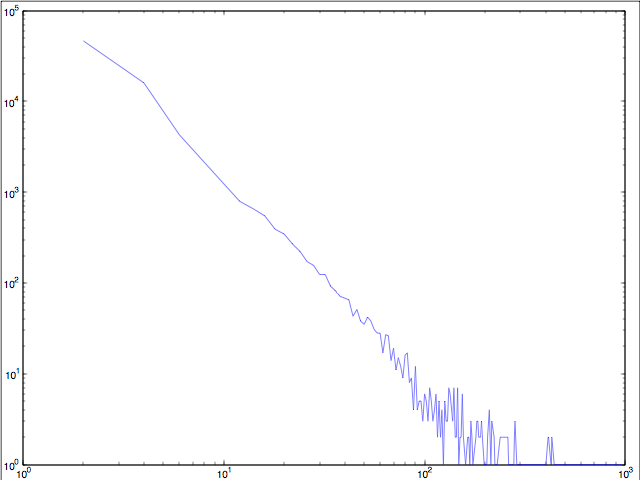
\includegraphics[width=.3\linewidth]{FIG/as-skitter.75000-indd.png}}\hfill
\subfloat[Out-Degree Distribution\label{fig:as-skitter_outdegree}]
  {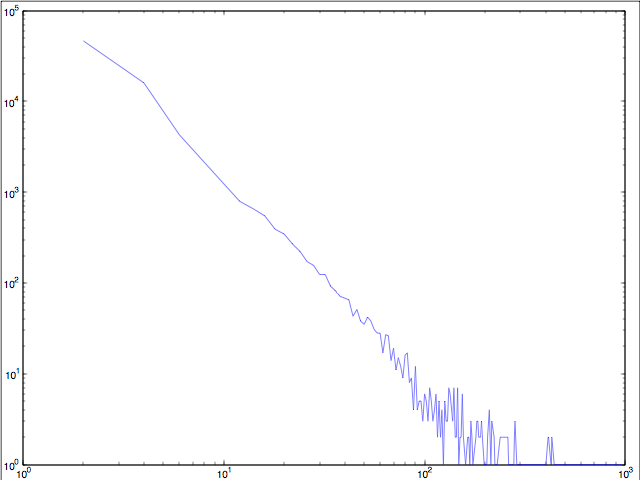
\includegraphics[width=.3\linewidth]{FIG/as-skitter.75000-outdd.png}}\hfill
\subfloat[Degree Distribution\label{fig:as-skitter_degree}]
  {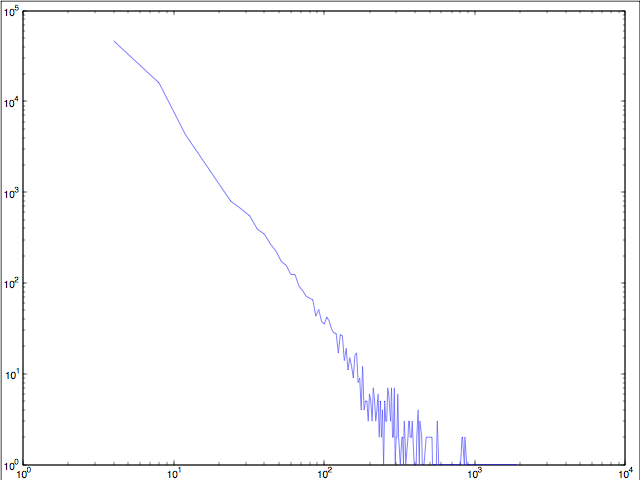
\includegraphics[width=.3\linewidth]{FIG/as-skitter.75000-dd.png}}
\caption{Degree Distributions of as-skitter\label{fig:as-skitter_degree_dist}}
\end{figure}
\subfloat[In-Degree Distribution\label{fig:ca-AstroPh_indegree}]
  {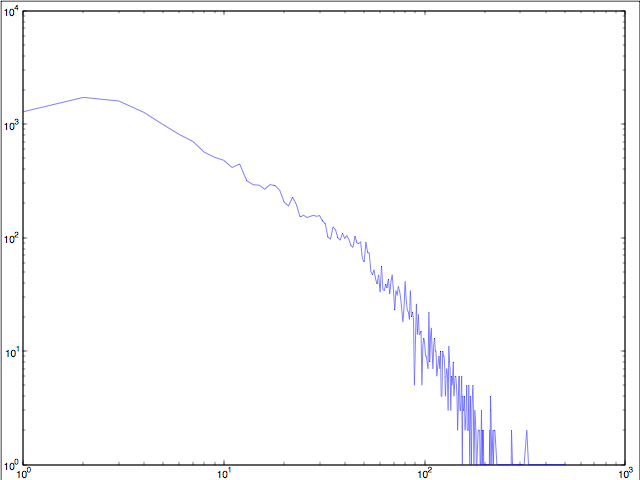
\includegraphics[width=.3\linewidth]{FIG/ca-AstroPh-indd.png}}\hfill
\subfloat[Out-Degree Distribution\label{fig:ca-AstroPh_outdegree}]
  {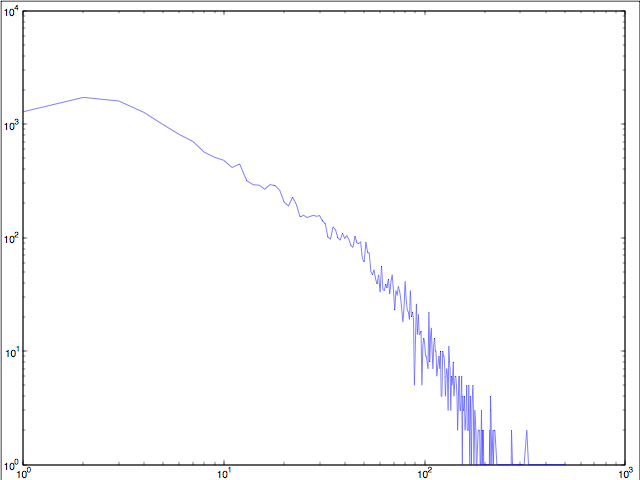
\includegraphics[width=.3\linewidth]{FIG/ca-AstroPh-outdd.png}}\hfill
\subfloat[Degree Distribution\label{fig:ca-AstroPh_degree}]
  {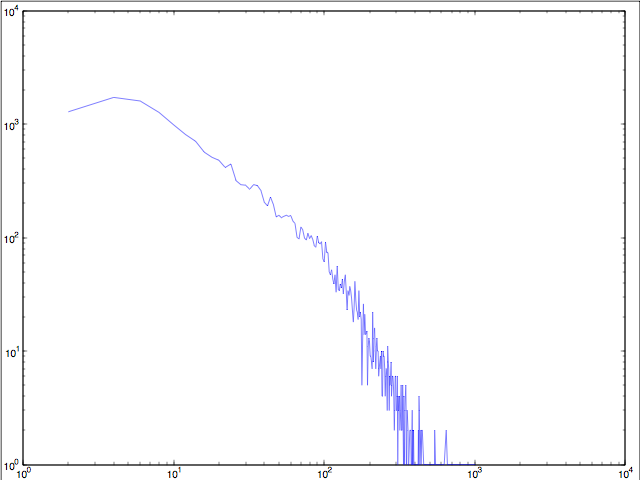
\includegraphics[width=.3\linewidth]{FIG/ca-AstroPh-dd.png}}
\caption{Degree Distributions of a-AstroPh\label{fig:ca-AstroPh_degree_dist}}
\end{figure}
\subfloat[In-Degree Distribution\label{fig:cit-HepPh_indegree}]
  {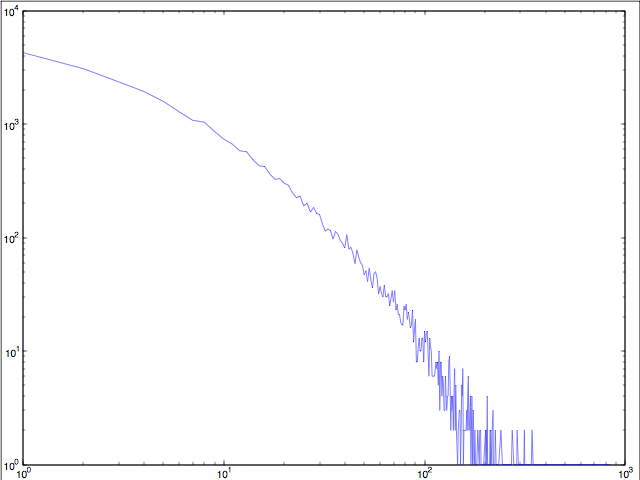
\includegraphics[width=.3\linewidth]{FIG/cit-HepPh-indd.png}}\hfill
\subfloat[Out-Degree Distribution\label{fig:cit-HepPh_outdegree}]
  {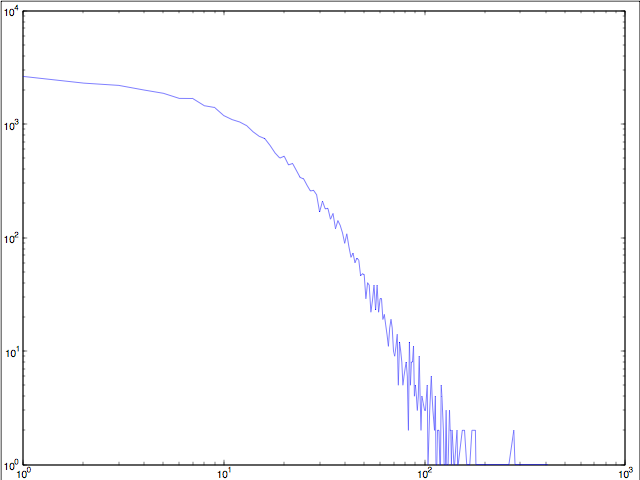
\includegraphics[width=.3\linewidth]{FIG/cit-HepPh-outdd.png}}\hfill
\subfloat[Degree Distribution\label{fig:cit-HepPh_degree}]
  {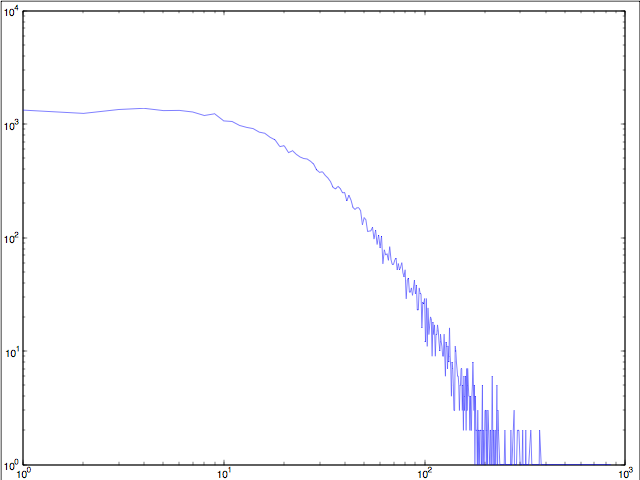
\includegraphics[width=.3\linewidth]{FIG/cit-HepPh-dd.png}}
\caption{Degree Distributions of cit-HepPh\label{fig:cit-HepPh_degree_dist}}
\end{figure}
\subfloat[In-Degree Distribution\label{fig:cit-HepTh_indegree}]
  {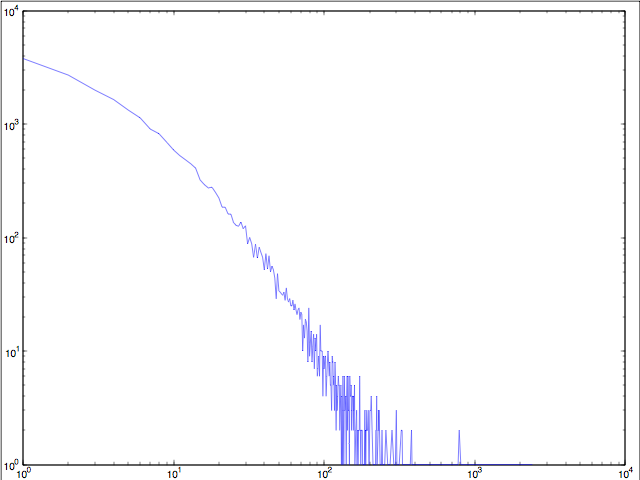
\includegraphics[width=.3\linewidth]{FIG/cit-HepTh-indd.png}}\hfill
\subfloat[Out-Degree Distribution\label{fig:cit-HepTh_outdegree}]
  {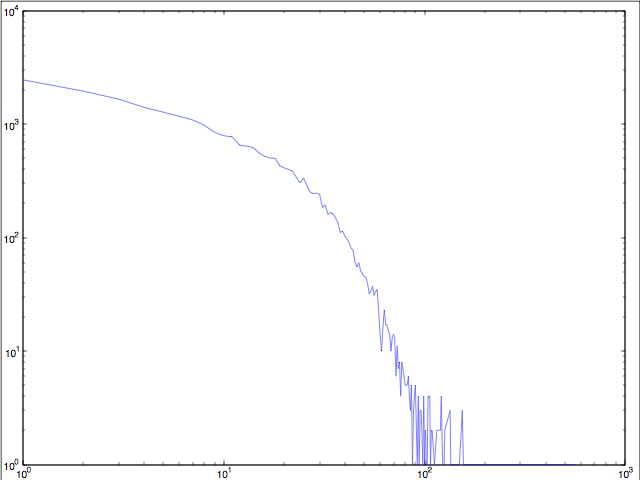
\includegraphics[width=.3\linewidth]{FIG/cit-HepTh-outdd.png}}\hfill
\subfloat[Degree Distribution\label{fig:cit-HepTh_degree}]
  {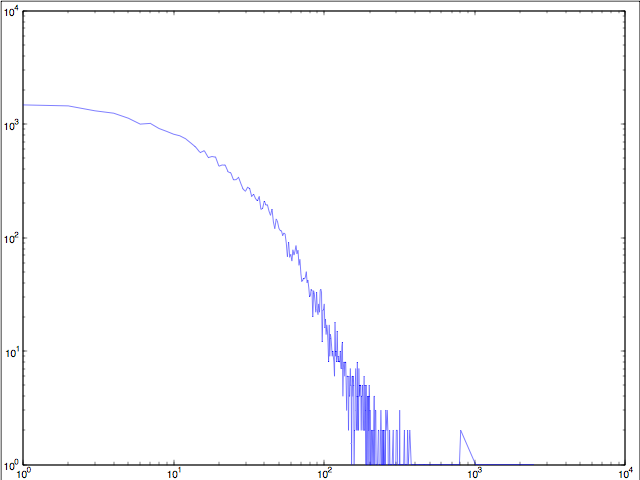
\includegraphics[width=.3\linewidth]{FIG/cit-HepTh-dd.png}}
\caption{Degree Distributions of cit-HepTh\label{fig:cit-HepTh_degree_dist}}
\end{figure}
\subfloat[In-Degree Distribution\label{fig:com-amazon.ungraph_indegree}]
  {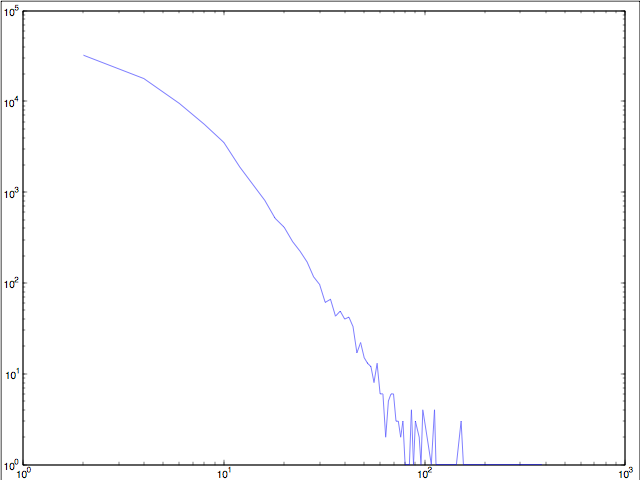
\includegraphics[width=.3\linewidth]{FIG/com-amazon.ungraph-indd.png}}\hfill
\subfloat[Out-Degree Distribution\label{fig:com-amazon.ungraph_outdegree}]
  {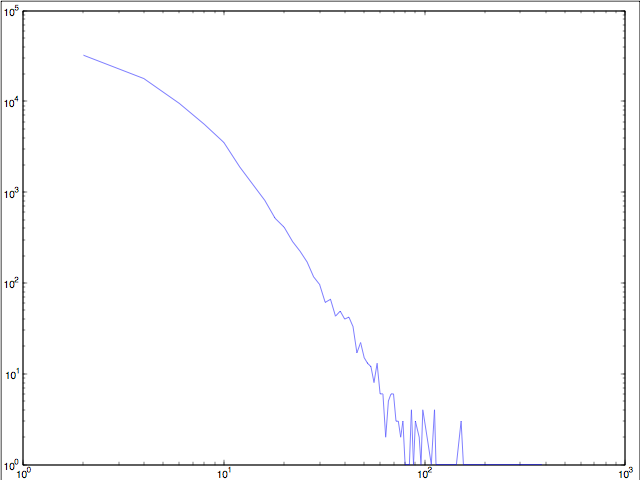
\includegraphics[width=.3\linewidth]{FIG/com-amazon.ungraph-outdd.png}}\hfill
\subfloat[Degree Distribution\label{fig:com-amazon.ungraph_degree}]
  {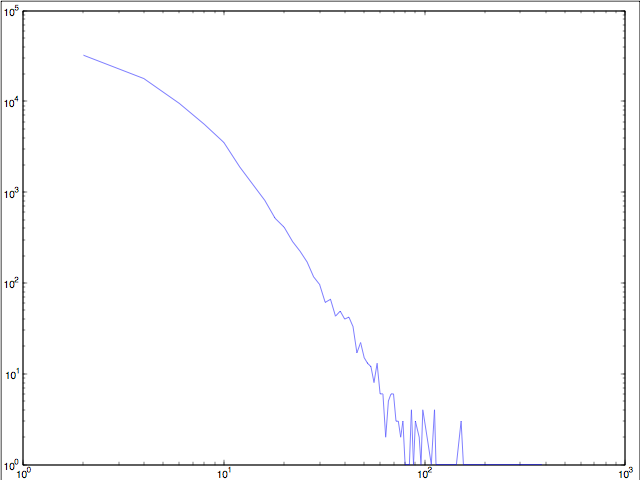
\includegraphics[width=.3\linewidth]{FIG/com-amazon.ungraph-dd.png}}
\caption{Degree Distributions of com-amazon.ungraph\label{fig:com-amazon.ungraph_degree_dist}}
\end{figure}
\subfloat[In-Degree Distribution\label{fig:com-dblp.ungraph_indegree}]
  {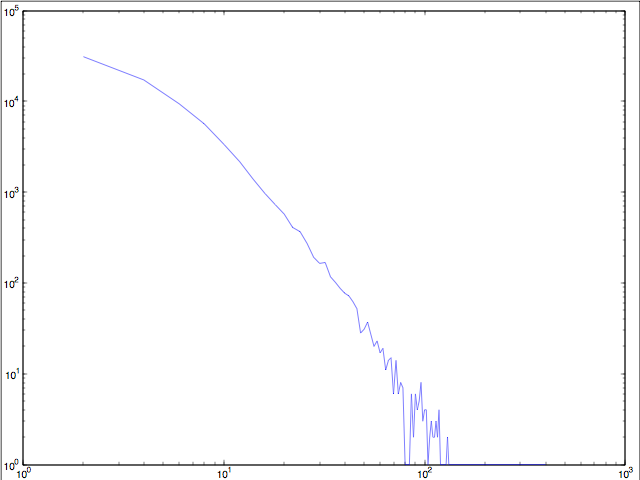
\includegraphics[width=.3\linewidth]{FIG/com-dblp.ungraph-indd.png}}\hfill
\subfloat[Out-Degree Distribution\label{fig:com-dblp.ungraph_outdegree}]
  {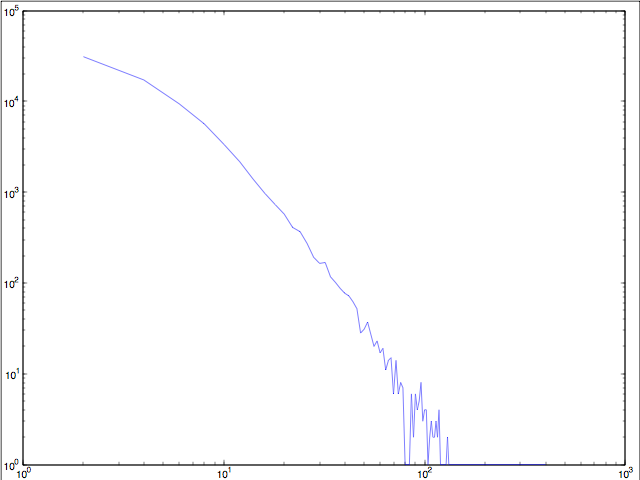
\includegraphics[width=.3\linewidth]{FIG/com-dblp.ungraph-outdd.png}}\hfill
\subfloat[Degree Distribution\label{fig:com-dblp.ungraph_degree}]
  {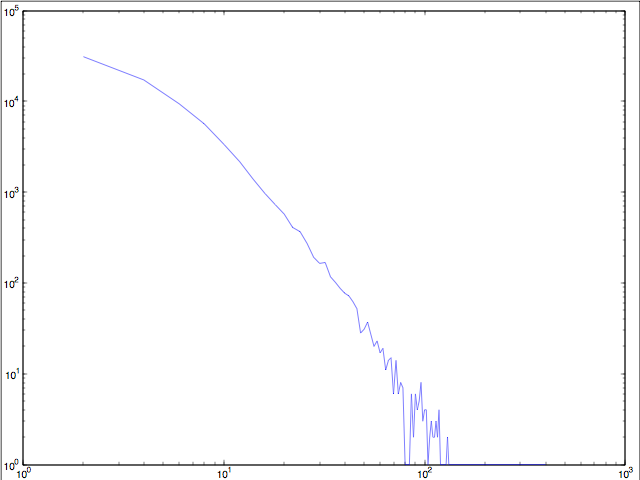
\includegraphics[width=.3\linewidth]{FIG/com-dblp.ungraph-dd.png}}
\caption{Degree Distributions of com-dblp.ungraph\label{fig:com-dblp.ungraph_degree_dist}}
\end{figure}
\subfloat[In-Degree Distribution\label{fig:email-Enron.ungraph_indegree}]
  {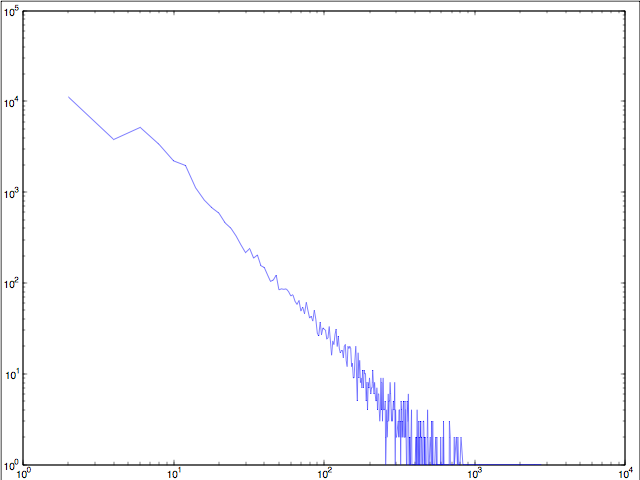
\includegraphics[width=.3\linewidth]{FIG/email-Enron.ungraph-indd.png}}\hfill
\subfloat[Out-Degree Distribution\label{fig:email-Enron.ungraph_outdegree}]
  {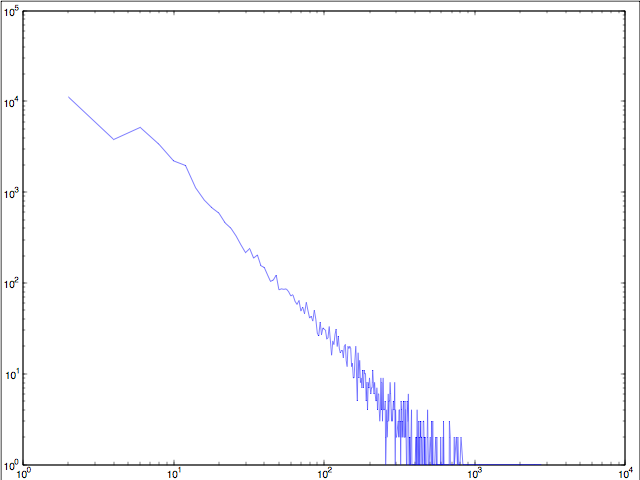
\includegraphics[width=.3\linewidth]{FIG/email-Enron.ungraph-outdd.png}}\hfill
\subfloat[Degree Distribution\label{fig:email-Enron.ungraph_degree}]
  {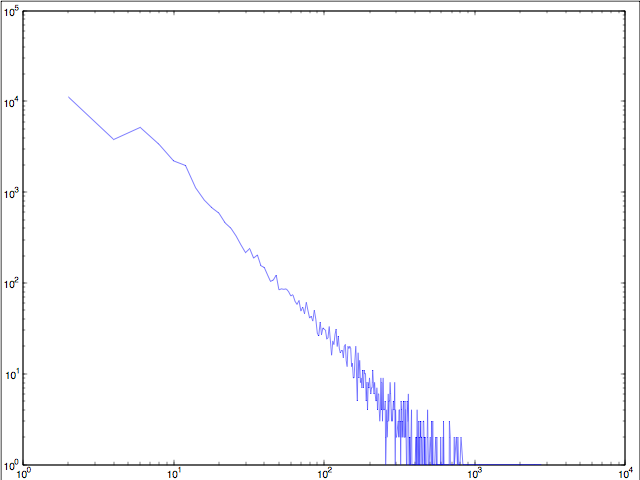
\includegraphics[width=.3\linewidth]{FIG/email-Enron.ungraph-dd.png}}
\caption{Degree Distributions of email-Enron.ungraph\label{fig:email-Enron.ungraph_degree_dist}}
\end{figure}
\subfloat[In-Degree Distribution\label{fig:email-EuAll_indegree}]
  {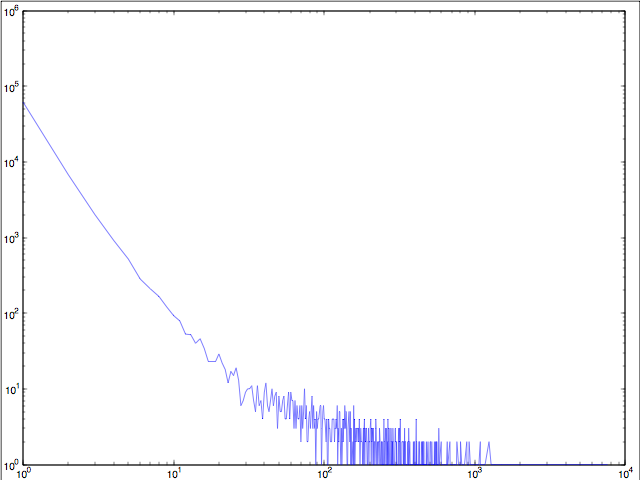
\includegraphics[width=.3\linewidth]{FIG/email-EuAll-indd.png}}\hfill
\subfloat[Out-Degree Distribution\label{fig:email-EuAll_outdegree}]
  {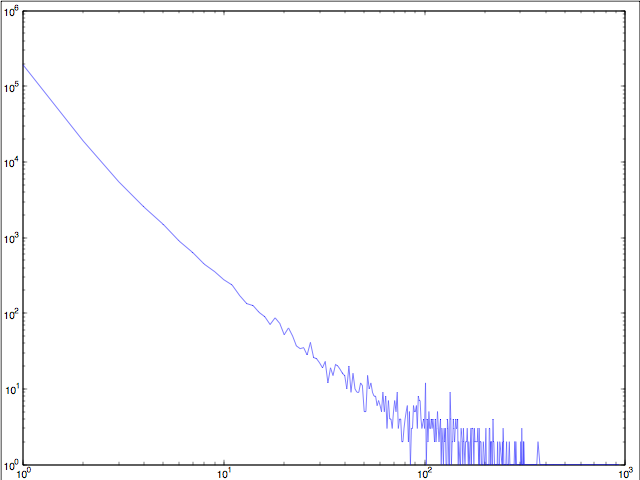
\includegraphics[width=.3\linewidth]{FIG/email-EuAll-outdd.png}}\hfill
\subfloat[Degree Distribution\label{fig:email-EuAll_degree}]
  {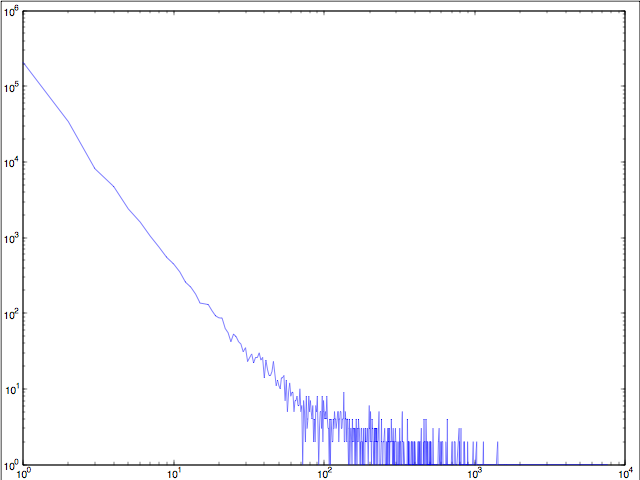
\includegraphics[width=.3\linewidth]{FIG/email-EuAll-dd.png}}
\caption{Degree Distributions of email-EuAll\label{fig:email-EuAll_degree_dist}}
\end{figure}
\subfloat[In-Degree Distribution\label{fig:p2p-Gnutella31_indegree}]
  {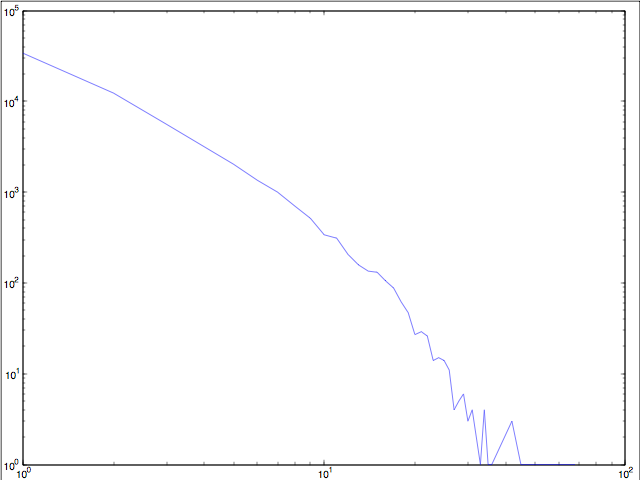
\includegraphics[width=.3\linewidth]{FIG/p2p-Gnutella31-indd.png}}\hfill
\subfloat[Out-Degree Distribution\label{fig:p2p-Gnutella31_outdegree}]
  {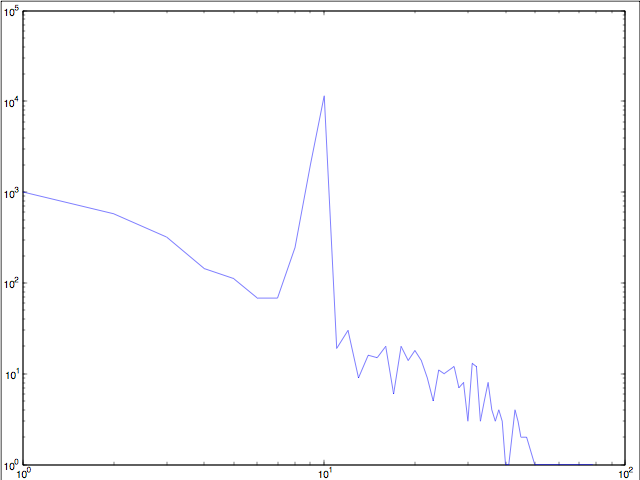
\includegraphics[width=.3\linewidth]{FIG/p2p-Gnutella31-outdd.png}}\hfill
\subfloat[Degree Distribution\label{fig:p2p-Gnutella31_degree}]
  {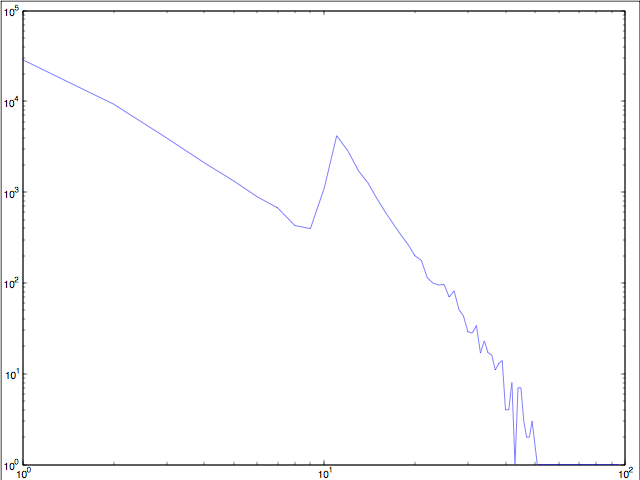
\includegraphics[width=.3\linewidth]{FIG/p2p-Gnutella31-dd.png}}
\caption{Degree Distributions of p2p-Gnutella31\label{fig:p2p-Gnutella31_degree_dist}}
\end{figure}
\subfloat[In-Degree Distribution\label{fig:soc-Slashdot0811_indegree}]
  {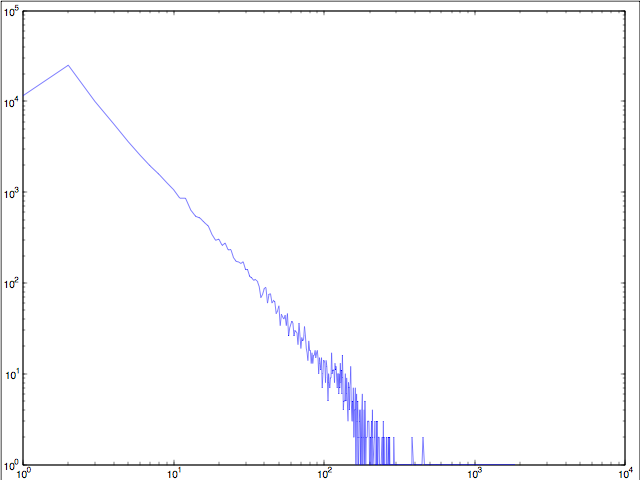
\includegraphics[width=.3\linewidth]{FIG/soc-Slashdot0811-indd.png}}\hfill
\subfloat[Out-Degree Distribution\label{fig:soc-Slashdot0811_outdegree}]
  {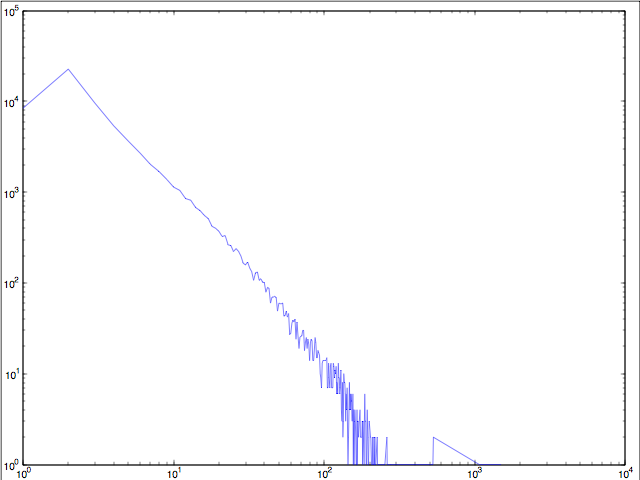
\includegraphics[width=.3\linewidth]{FIG/soc-Slashdot0811-outdd.png}}\hfill
\subfloat[Degree Distribution\label{fig:soc-Slashdot0811_degree}]
  {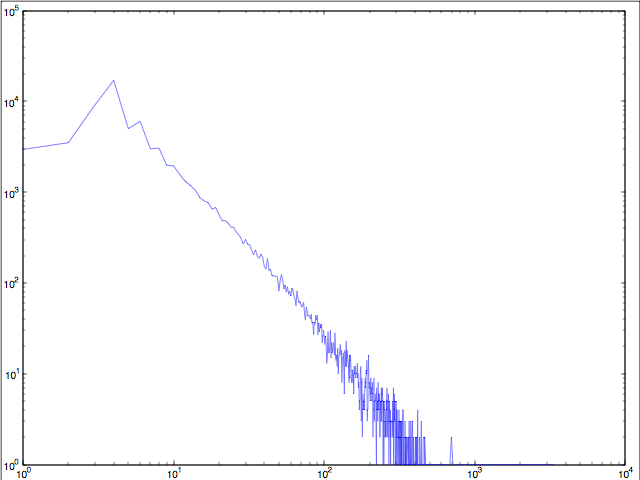
\includegraphics[width=.3\linewidth]{FIG/soc-Slashdot0811-dd.png}}
\caption{Degree Distributions of soc-Slashdot0811\label{fig:soc-Slashdot0811_degree_dist}}
\end{figure}
\end{document}